\documentclass[10pt, reqno]{article}
\usepackage[left=3cm,right=3cm,top=3cm,bottom=3cm]{geometry}
\geometry{letterpaper}                   
\usepackage[utf8]{inputenc}
\usepackage[numbers]{natbib}
\usepackage{graphicx}
\usepackage{color}
\usepackage{amssymb}
\usepackage{verbatim}
\usepackage{amsmath}
\usepackage{epstopdf}
\usepackage{enumerate}
\usepackage[format=plain,font=footnotesize,labelsep=newline,singlelinecheck=false,justification=justified,margin=1cm]{caption}
\DeclareGraphicsRule{.tif}{png}{.png}{`convert #1 `dirname #1`/`basename #1 .tif`.png}
\setlength{\parindent}{25pt}
\renewcommand{\abstractname}{}

\title{Python calculations of Bohmian trajectories}
\author{Dane Odekirk} 
\date{October 28th, 2012}                                         


\begin{document} 
\maketitle 
\pagebreak

\begin{abstract}
  \noindent 
  {\bf Abstract. } 

  %[TODO: SEPARATE SYSTEMS IS NOT CORRECT SINCE ITS BOTH 2 INTERFEREING WAVE PACKETS. RELATED SYSTEMS IS BETTER]
  The Python programming language is used to calculate Bohmian trajectories for two interfering wave-packets. 
  A fourth-order Runge-Kutta is implemented to numerically solve the differential equations that describe the trajectories.
  Trajectories are computed on a 1.7Ghz Core i5 processor using Python version 2.7.2 with the NumPy, SymPy and Matplotlib packages.
  All results agree with current de Broglie-Bohm theory.
  The Python scripts are referenced in the appendix.

\end{abstract}




\section{Introduction}

  Quantum mechanics is famed for introducing uncertainty to a once certain world.
  %The causal determinism of everyday experience is lost within its statistical foundation.
  The de Broglie-Bohm theory rectifies this with a causal interpretation of quantum mechanics by 
    prescribing definite trajectories to particles without sacrificing predictive accuracy.
  %[TODO: THIS IS DUPLICATED. SAY IT ONCE]
  This is a stark contrast to the Copenhagen interpretation where a system's behavior is nondeterministic.  
  The ramifications of the de Broglie-Bohm interpretation remedy the concept of wave-particle duality since
    quantum systems can be predicted without losing the particles.
  This gives rise to a narrative of the particles that can be discussed, analyzed and is not hidden nor ignored as it with 
    the Copenhagen interpretation.

%  Solving the Schrödinger equation with the wave function expressed in Euler form yields a result that describes 
%    these trajectories and how the quantum potential emerges.
  The de Broglie-Bohm theory proposes that a system of $n$ particles has trajectories described by 

  \begin{equation} \label{eq:trajectories}
    \dot{r} = \frac{\hbar}{m_i}\text{Im}[\frac{ \nabla_{i} \Psi(r_1,\dots,r_n,t)}{\Psi(r_1, \dots, r_n, t) } ]
  \end{equation}

  \noindent
  for each particle $i$; where $\Psi$ is the total wave function \cite{guay}.
  This is recognized as the guiding equation.
  First presented by de Broglie in 1927, the de Broglie interpretation of quantum mechanics was quickly abandoned after a confident rebuttal by Pauli during a conference.
  Although de Broglie's defense was accurate, Pauli and his objections garnered support and momentum away from the de Broglie interpretation
    and it was eventually abandoned as the Copenhagen interpretation became more popular.
  In 1952, however, Bohm reintroduced the theory with proper rebuttals of Pauli's objections \cite{bohm}.

  Bohm's theory, also known as Bohmian mechanics or de Broglie-Bohm theory, is formulated via the Schrödinger equation \cite{bohm}.
  To illustrate, consider the one-particle Schrödinger equation given by 
    \begin{equation}
      i \hbar \frac{\partial}{\partial t} \Psi(\mathbf{r},t) = \Bigg[ \frac{-\hbar}{2m} \nabla^2 + V(\mathbf{r},t) \Bigg] \Psi(\mathbf{r},t)
    \end{equation}
  where $V$ is the potential and $\Psi$ is the wave function.
  When the wave function is written in Euler form 
    \begin{equation}
      \Psi(\mathbf{r},t) = \sqrt{P} \exp(\frac{iS}{\hbar}) 
    \end{equation}
  where $P$ and $S$ are real, dimensionless functions, the Schrödinger equation can be evaluated.
  Separating the result into real and imaginary parts yields the following equations:
  \begin{align} 
    \frac{\partial P}{\partial t} &= - \mathbf{\nabla} \cdot (P \frac{\mathbf{\nabla} S}{m}) \label{eq:bohm1} \\
    %\frac{\partial S}{\partial t} &= - \frac{1}{2}( \mathbf{\nabla}S^2 - Q - V(\mathbf{r}) \label{eq:bohm2} )
    \frac{\partial S}{\partial t} &= - \frac{1}{2} \Bigg[ \frac{(\nabla S)^2}{m} - 2V(\mathbf{r}) + Q \label{eq:bohm2} \Bigg] 
  \end{align}
  where Q is given by
  \begin{equation} \label{eq:quantumpotential}
    Q = -\frac{\hbar^2}{2m}\frac{\nabla^2 \sqrt{P}}{\sqrt{P}}
  \end{equation}
  %Refer to reference \cite{bohm} for a more in-depth derivation of these equations.
  %[todo: put this somewhere else?] 
  For the remainder of this paper, the constants $m$ and $\hbar$ are set equal to one.
    
  Bohm recognized when evaluating equation (\ref{eq:bohm1}) at the classical limit, $ \hbar \rightarrow 0 $, 
    that $S$ is the solution to the classical Hamilton-Jacobi equations of motion \cite{bohm}.
  %When the classical limit is approached the function $Q$ approaches zero as it is dependent on $\hbar$.
  The Hamilton-Jacobi equations are accurate for classical systems, however,
    are incomplete for the quantum realm.
  Specifically, the function $Q$ approaches zero classically and only exists at the quantum limit.
  %This is reminiscent of the theory of special relativity, in which the Taylor expansion of energy yields the traditional
  %  equation for kinetic energy as an infinite series; thereby, turning the traditional equation into a basic approximation.
  %In terms of de Broglie-Bohm theory, solving the Schrödinger equation in Euler form is analogous to the Taylor expansion and 
  %  the Hamilton-Jacobi equations of motion are the basic approximation.
  This function $Q$ is known as the quantum potential and is the difference between the quantum and classical Hamilton-Jacobi equations of motion.
  It also plays a significant role in the behavior of de Broglie-Bohm particle trajectories.
  Bohm quotes the following theorem \cite{bohm} 
  \begin{quotation}
    \noindent
    If we consider an ensemble of particle trajectories which are solutions of the equations of motion,
    then it is a well-known theorem of mechanics that if all these trajectories are normal to any given surface of constant $S$,
    then they are normal to all surfaces of constant $S$, 
    and $\nabla S(x) / m $ will be equal to the velocity vector, $\mathbf{v}(\mathbf{x})$,
    for any particle passing the point $ \mathbf{x} $.
  \end{quotation}
  Applying this theorem yields two results.
  First, equation (\ref{eq:bohm1}) can be rewritten in terms of a particle's velocity since $\nabla S(x)$ is equal to the velocity $\mathbf{v}$.
    %, where the particles $m$ is equal to one. 
  P is therefore consistent with the probability density for these particles,
    where $P\mathbf{v}$ represents the mean current of particles.
  %When this substitution is made the function $P$ [TODO: BECOMES IS BAD WORD CHOICE. 'IS' IS BETTER] becomes consistent with the probability density for these particles, where $P\mathbf{v}$ represents the mean current of particles.
  Equation (\ref{eq:bohm1}) then represents the conservation of probability.
  Second, equation (\ref{eq:bohm2}) is consistent with the Hamilton-Jacobi for a system of such particles.
  Unlike its classical counterpart, however, the particles are affected by two types of potentials: 
    the classical potential $V$ and the quantum potential $Q$.
  %This is the basic foundation for the de Broglie-Bohm interpretation of quantum mechanics.

  To summarize, solving the Schrödinger equation with a wave function in Euler form results in a set of equations.
  These set of equations are equal to the Hamilton-Jacobi equations of motion at the classical limit 
    and introduce the new quantum potential $Q$ at the quantum limit.
  Furthermore, they imply a set of calculable trajectories for each particle in the system;
    defining a narrative that is nonexistent in the Copenhagen interpretation.
  %These trajectories are governed by both the classical potential $V$ the quantum potential $Q$.

  In order to calculate Bohmian trajectories of a particle, its $x$ and $y$ position must be determined at any given time $t$.
  The $x$ component of the particle's position can be found via 
  \begin{equation}
    x(t) = x(0) + k_x t 
  \end{equation}
  where $k_x$ is the velocity in the $x$ direction \cite{guay}.
  This simplifies the calculation by allowing us to focus specifically on the $y$ coordinate realizing that 
    the $x$ coordinate is simply proportional to the time $t$.
  %In terms of plotting the trajectories the change in $y$ position over time must be found out, while the 
  %  change in the $x$ position is a known, equal spacing between each interval of time.
  The $y$ coordinate of a particle at time $t$ is found by feeding the wave function $\Psi$ that describes the system into equation (\ref{eq:trajectories}).
  With initial random values of $t_0$ and $y_0$, equation (\ref{eq:trajectories}) is evaluated over iterations of times $t$ between $t_i$ and $t_f$ to calculate the 
    particle's $y$ coordinate at each specific time $t$.
  Compiling this solution with the $x$ coordinate yields the trajectory of a particle with initial position $x_0$ and $y_0$.
  %When these calculations are iterated over an interval of time, specific coordinates for each time $t$ is found and consequentially a trajectory.
  %As mentioned previously, the Runge-Kutta algorithm was used for two reasons: the error analysis \cite{rungekutta} and the results display trajectories
  %  that follow the theoretical characteristics of Bohmian trajectories. 
  %The second reason is more subjective then the first, however, nonetheless important.
  %If, for example, the Runge-Kutta algorithm smoothed out trajectories and removed the effects of the quantum potential it would not be used.
  %Fortunately, a fourth-order Runge-Kutta algorithm works for our desired results.
  
  In this paper a fourth-order Runge-Kutta is implemented to compute the Bohmian trajectories defined by equation (\ref{eq:trajectories}) \cite{dowsa}.
  Interfering wave packets are investigated for two related systems.
  Python 2.7.2 is the programming language of choice because of its syntax, built in debugger, and open-sourced scientific packages.
  The language itself is freely available and open-sourced as well.
  The specific packages used are NumPy, SymPy and Matplotlib which provide numerical functions, symbolic math and plotting functions respectively.
  Full understanding of these packages is not necessary to understand or run the Python code; 
    although some background knowledge of their capabilities, purposes and implementations could prove helpful.

  %numerically since the Runge-Kutta is more accurate when compared to alternative methods [TODO: EXPAND ON THIS. CITE THE METHODS WHY ONE IS CHOSEN OVER THE OTHER] \cite{rungekutta}; specifically in the context of Bohmian trajectories.

%  The results of Bohmian mechanics should be indistinguishable from quantum mechanics and this has been the case insofar.
%  Even though Bohmian mechanics introduce trajectories - specific position and velocity for each particle - the theory's [TODO: DUPLICATE. SAY IT ONCE] predictions
%    are still statistical in nature even though the system's behavior is causal.
%  It is debated whether this is a weakness in the theory since all the theory provides is a different means to the end, 
%    however this discussion is not the purpose of this paper.
%
%  Bohmian trajectories will first be calculated for the double-slit experiment.
%  This will provide a foundation for the Python implementation since the results of the double-slit experiment are well established.
%  Once the results are corroborated the same technique will be applied to [TODO: THIS IS INCORRECT. RELATED NOT SEPARATE SYSTEMS] two interfering wave packets; thereby finding the Bohmian trajectories for this system.
%  A fourth-order Runge-Kutta method will be implemented to solve equation (\ref{eq:trajectories}) numerically since the Runge-Kutta is more accurate when compared to alternative methods [TODO: EXPAND ON THIS. CITE THE METHODS WHY ONE IS CHOSEN OVER THE OTHER] \cite{rungekutta}; specifically in the context of Bohmian trajectories.
%  %The results of these calculations will be directly affected by the decision to use Runge-Kutta over alternatives.
%  A three-dimensional representation of the wave functions for both systems will be graphed to clarify how Bohmian trajectories behave in these systems. 
%  This will provide a [TODO: UNIQUE IS A BAD WORD CHOICE] unique perspective on the underlying wave functions that eventually determine the path of the Bohmian trajectories.
%  Furthermore, the trajectories for both systems will be plotted and discussed.
%
%  A final note, the Python programming language is chosen because it is free, open-sourced and capable of necessary numerical analysis.
%  In order to achieve the calculation of Bohmian trajectories a set of packages will be utilized: NumPy, SymPy and Matplotlib.
%  All of which will be necessary dependencies of the Python code.
%  These packages provide powerful utilities that will be used to graph the wave functions and calculate the Bohmian trajectories for both systems.
%  Note that full understanding of these packages is not necessary to understanding or run the Python code; although some background information on their capabilities, purposes and implementations could prove helpful.




\section{Double-slit experiment}

  Bohmian trajectories are calculated for a double-slit setup.
  The classical double slit experiment consists of the following parts:
    a source that emits particles,
    a barrier with two slits A and B cut into it,
    and a screen that captures and records the particles.
  This is illustrated in Figure \ref{fig:double-slit}.
  The system implemented in this investigation shares these characteristics and makes no special alterations to the traditional experimental setup.

  \begin{figure}[!ht]
    \centerline{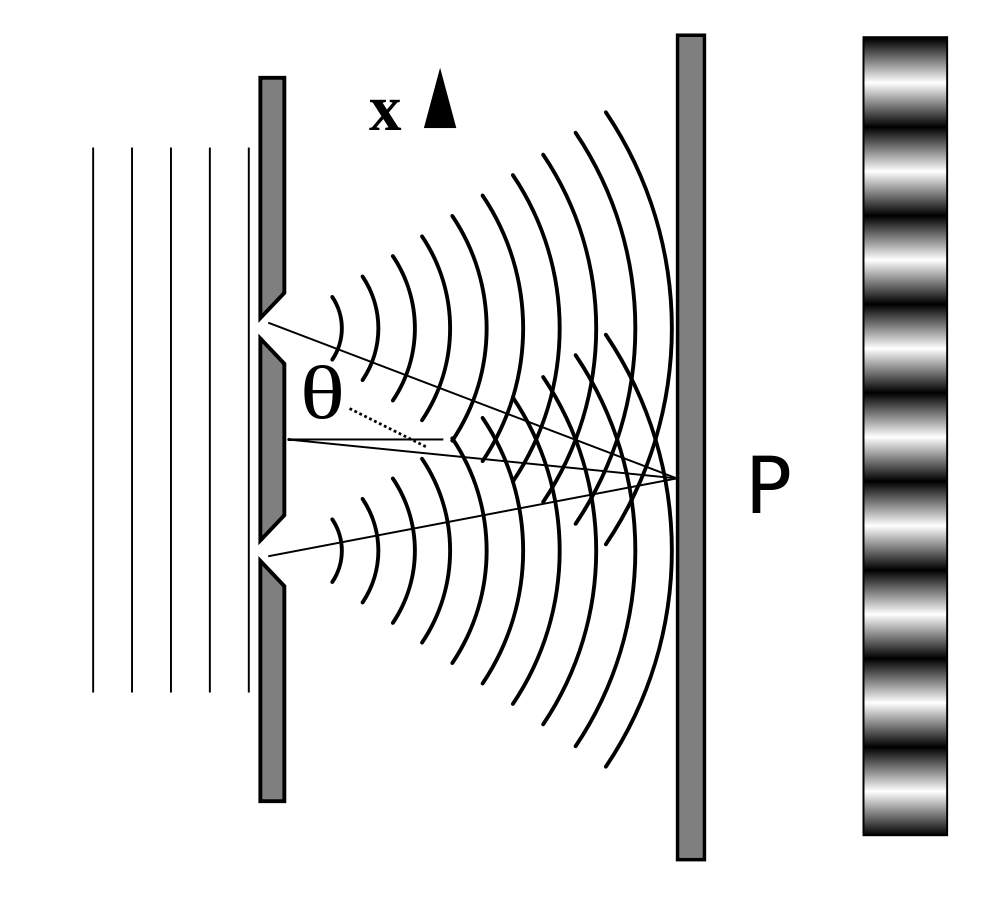
\includegraphics[scale=.2]{./imgs/double-slit.png}}
    \caption{
      Traditional double slit setup \cite{wiki}. 
      Bohmian trajectories are calculated for such a system.
    }
    \label{fig:double-slit}
  \end{figure}

  %[TODO: SHOW FIGURES OF BOTH SETUPS INSTEAD OF THE EQUATIONS HERE. THE DOUBLE SLIT AND DOUBLE REFLECTION]
  When a particle goes through either slit its wave function is described by $\psi_A(\mathbf{r},t)$ and $\psi_B(\mathbf{r},t)$ for slits A and B respectively.
  %The symmetry of the system allows us to make the [TODO: ASSUMPTION IS NOT GOOD. REMOVE EQUATION. STATE IT BUT RECALL THAT REALITY IS NOT SYMMETRICAL] following assumption
  %\begin{equation}
  %  \psi_A(\mathbf{r_x},\mathbf{r_y},\mathbf{r_z},t) = \psi_B(\mathbf{r_x}, -\mathbf{r_y},\mathbf{r_z},t)
  %\end{equation}
  %which illustrates that each partial wave function $\psi_A$ and $\psi_B$ are transforms of each other over the x-axis.
  The wave that leaves the slit has an exact solution described by the following time-dependent equation \cite{guay-double-slit}
  \begin{equation}
    \label{eq:partial}
    \psi_n(\mathbf{r},t) = (2\pi\sigma^2)^{-1/4} \exp \Bigg[ \frac{(y_i - Y)^2}{4 \sigma_{0} \sigma_{t}} + i \Bigg[ k_x x_i - \frac{k_x^2 t}{2} \Bigg]\Bigg]
  \end{equation}
  where 
  \begin{equation}
    \sigma_{t} = \sigma_{0}(1 + \frac{it}{2\sigma^2_0})
  \end{equation}
  This definition assumes the particles are traveling in free space and the classical voltage $V$ is zero.
  The total wave function needed to calculate trajectories with equation (\ref{eq:trajectories}) is described by the following equation
  \begin{equation}
    \label{eq:total-wave-function}
    \Psi(\mathbf{r},t) = N [\psi_A + \psi_B ]
  \end{equation}
  where $\psi_A$ and $\psi_B$ are defined by equation (\ref{eq:partial}) and $N$ is a normalization constant.
  % [TODO: REMOVE THIS SENTENCE] There is nothing significantly unique about this wave function as it follows the same pattern of any typical time-dependent wave equation in quantum 
    %mechanics.

  Figures \ref{fig:2d0} and \ref{fig:2d1} illustrate the time-dependence of the wave function $\Psi$.
  Both the real and imaginary parts of of the wave function, described by equation (\ref{eq:total-wave-function}), are plotted at times $t=0$ and $t=1$. 
  %Please refer to the appendix for a larger version of this image and all further images in this article.
  Both Figures \ref{fig:2d0} and \ref{fig:2d1}, span $y$ values from -13 to 13 with a spacing of 0.01, accounting for 2600 points to be plotted.
  Good consistency is found between these figures and figures in reference \cite{guay-double-slit} on which these graphs are based.
  The code to produce these figures is shown in appendix \ref{appendix:real-imag}.
 %   being the first step in corroborating the correctness of the Python implementation of the wave function.
 % The code necessary to generate these figures are coupled with the figures themselves in the appendix. 
 % There are a few things to note. 

    \begin{figure}[!ht]
      \centerline{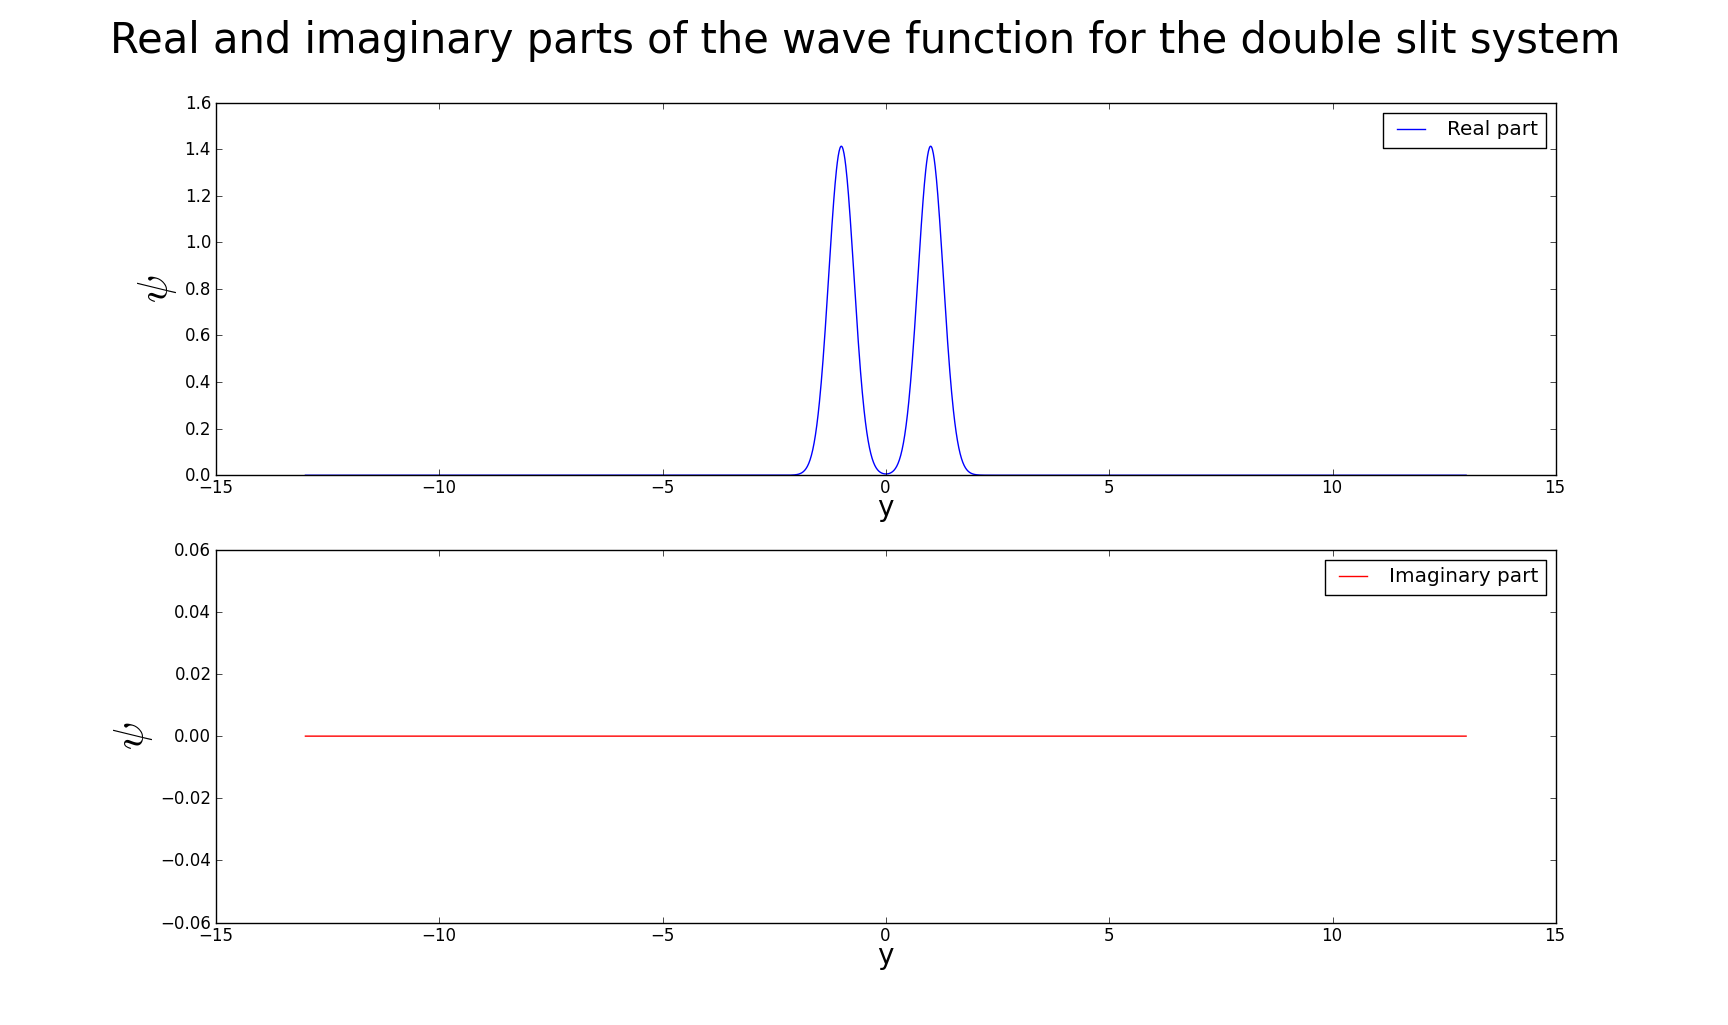
\includegraphics[scale=.3]{./imgs/double-slit-real-imaginary-parts-t0.png}}
      \caption{
        Two-dimensional breakdown of the real (blue) and imaginary (red) parts of equation (\ref{eq:total-wave-function}) evaluated at $t=0$.
        Values of $y$ span from -13 to 13 with spacing $\Delta y$ of 0.01.
      }
      \label{fig:2d0}
    \end{figure}
    \begin{figure}[!ht]
      \centerline{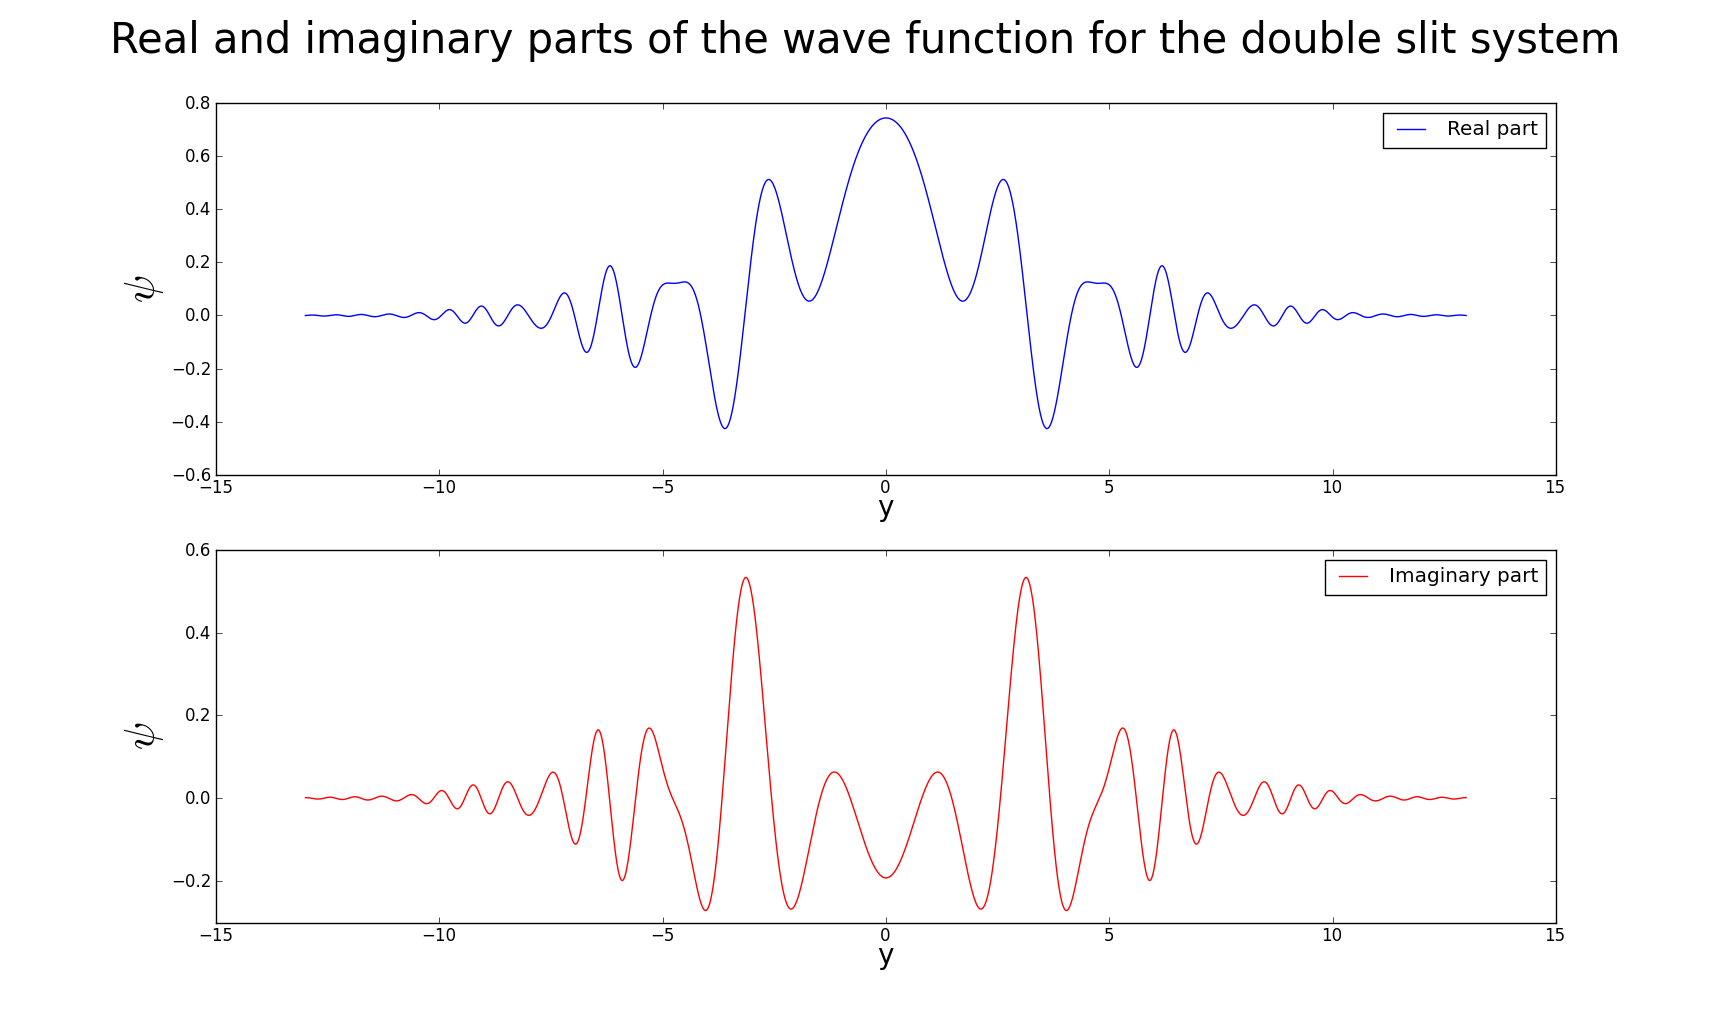
\includegraphics[scale=.3]{./imgs/double-slit-real-imaginary-parts-t1.png}}
      \caption{
        Two-dimensional breakdown of the real (blue) and imaginary (red) parts of equation (\ref{eq:total-wave-function}) evaluated at $t=1$.
        Values of $y$ span from -13 to 13 with spacing $\Delta y$ of 0.01.
      }
      \label{fig:2d1}
    \end{figure}

  According to equation (\ref{eq:trajectories}) the imaginary part of the wave function plays an important role in guiding particles along their 
    Bohmian trajectories.
 % As shown in Figures \ref{fig:2d0} and \ref{fig:2d1}, there is a [TODO: WHAT DOES THIS MEAN? IS IT IMPORTANT UGH TO KEEP?] 
 %   change in the imaginary part of the wave function over time and it is this change that [TODO: WHAT DOES THIS MEAN? KEEP IT?] directly affects the trajectories.
  For a more revealing perspective, the imaginary part of the wave function is plotted three-dimensionally over time in Figure \ref{fig:3d}
    with a color grading representing the gradient along its surface.
  Note that the $x$ axis has been replaced by the time $t$ as they are proportional to one another.
  %This reasoning will be explained more explicitly shortly.
  Values for $y$ once again span between -13 and 13 with a spacing of 0.01 and
    values for $t$ span between 0 and 1 with a spacing of 0.01.
  These values are chosen on a rather subjective basis of time - as decreasing the spacing increases the computation time.
  Generating Figure \ref{fig:3d} takes approximately 1.35 seconds with the given values.
  The code to generate this graph is shown in appendix \ref{appendix:imaginary-surface}.
  %[TODO: REMOVE THIS SENTENCE] Unfortunately, only one view can be shown in this article, but the graph itself can be manipulated to different points of view by running its corresponding Python code.
  %[TODO: MAKE THIS FIGURE AND OTHERS BIGGER. REMOVE APPENDIX]

  Figure \ref{fig:3d} clarifies the underlying mechanisms that govern the Bohmian trajectories.
  Notice the imaginary parts of Figures \ref{fig:2d0} and \ref{fig:2d1} agree with the cross-section parallel to $x$ of Figure \ref{fig:3d} at times $t=0$ and $t=1$.
  %The imaginary part of the wave function for different times $t$ can also be found within Figure \ref{fig:3d} by merely taking the cross-section of the surface for different values of $t$.
  %More importantly, however, is how much this Figure \ref{fig:3d} highlights how Bohmian trajectories behave.
  %Metaphorically, if one would imagine pushing a ball from $t=0$ towards $t=1$, the path the ball
  %  would take would be entirely dependent on the surface it travels.
  The crest and troughs of the wave function govern the direction of the particle. 
  Higher crests require higher energy while the troughs require lower energy.
  The trajectories follow the path of lowest energy.
  Not depicted in Figure \ref{fig:3d} is the quantum potential $Q$ that also affects the trajectories - it is plotted in reference \cite{bohm}. 
  When $Q$ is plotted three-dimensionally, it also illustrates the crests and troughs that govern the particle's trajectory \cite{bohm}.
  %In the case of Figure \ref{fig:3d}, the crests and troughs at $t=1$ would represent where most particles would find themselves by the time they reached the screen.

  Of more interest, however, is the concept of the trajectory. 
  The narrative behind the Copenhagen interpretation is one that focuses on predictions and observations while ignoring how the observation came to be.
  With the de Broglie-Bohm interpretation, the prediction is still valid however the particle's trajectory, or the history of how it arrived at the observation, 
    can still be calculated and discussed.
  %The changing landscape of the surface would result in trajectories that do not simply go straight, but instead wind their ways around the crests.
  %The predicted trajectories based on analyzing the shape and surface of Figure \ref{fig:3d} insofar agree with the characteristics of Bohmian trajectories.
  %[TODO: EXPAND ON THIS BELOW]
  %There is an assumption here, but it is one of the many put forth by the Bohmian interpretation.
  For example, the de Broglie-Bohm interpretation shows that a particle does in fact go through a specific slit; either one or the other.
  It does not have a predictive measure to calculate which slit the particle will go through prior to reaching the slits, however, does define 
    a historical trajectory that leads to a single, specific slit.
  This is not the case in the Copenhagen interpretation where 
    the particle's probability wave passes through both slits and the concept of a physical particle passing through a single slit is irrelevant.


    \begin{figure}[!ht]
      \centerline{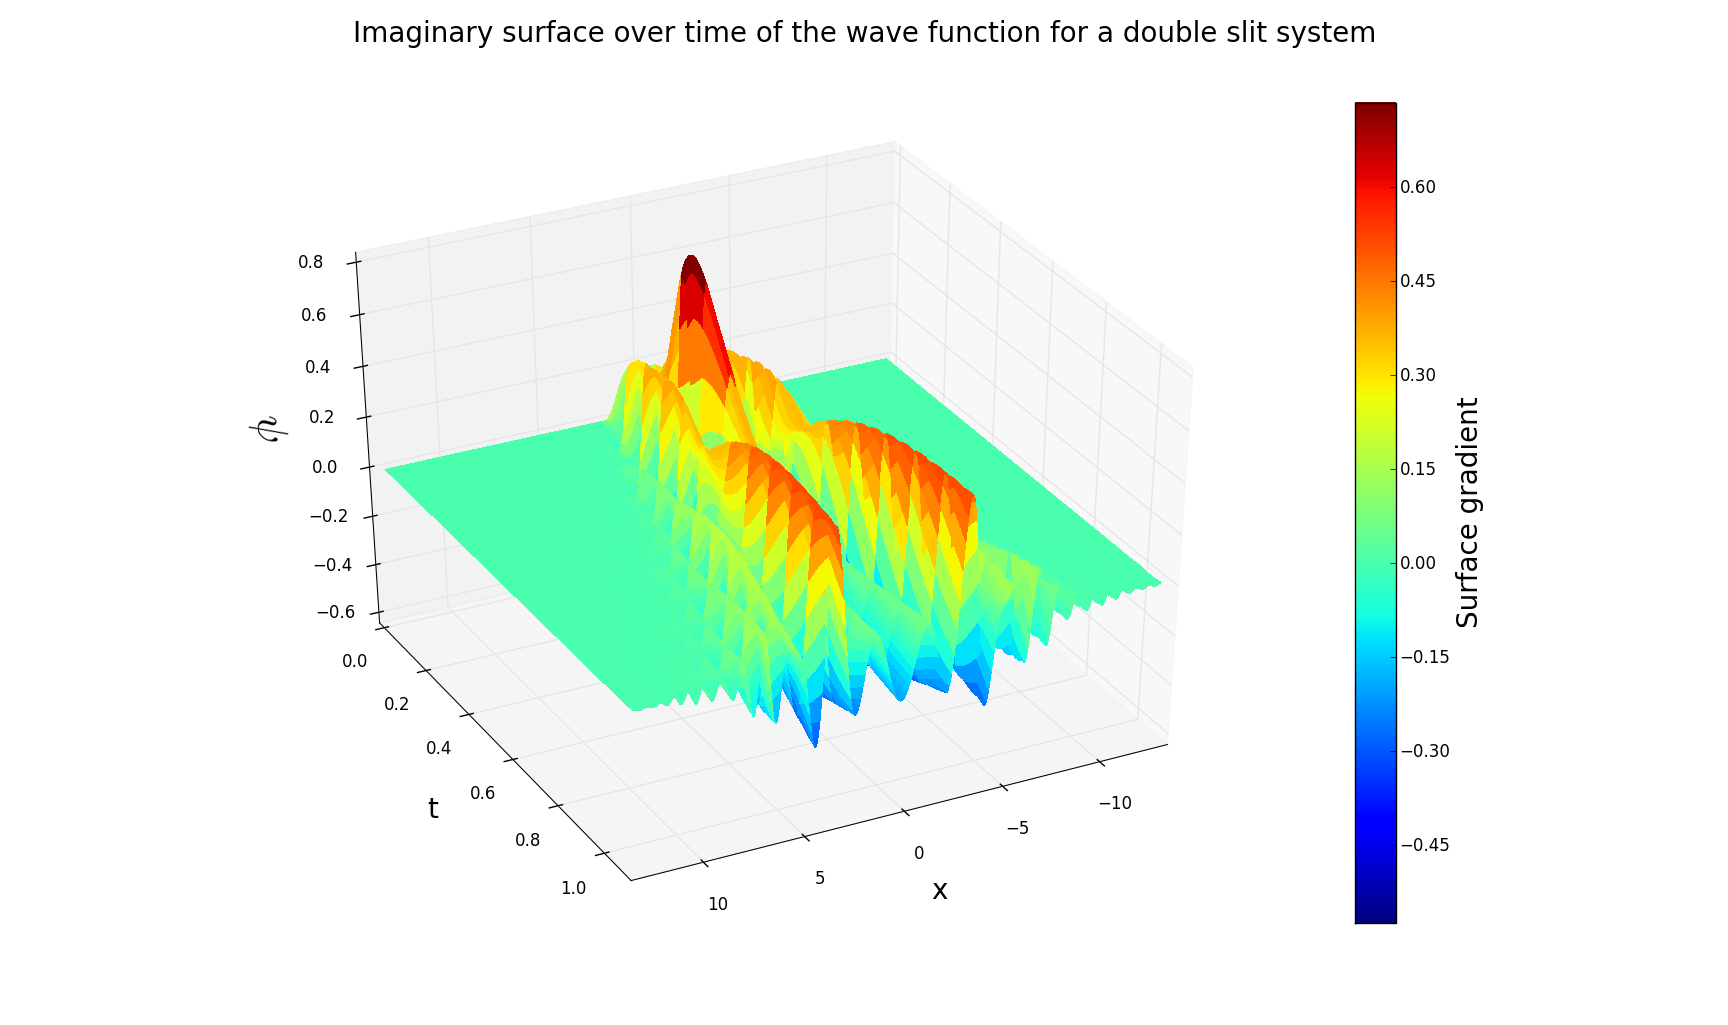
\includegraphics[scale=.4]{./imgs/double-slit-real-imaginary-parts-3d.png}}
      \caption{
        Three-dimensional plot of the imaginary surface of equation (\ref{eq:total-wave-function}) as it propagates through time.
        This figure exposes the physical importance of the wave function, which inevitably governs the path of particles at they traverse from $t=0$
      to $t=1$.
      }
      \label{fig:3d}
    \end{figure}

\section{Double-slit trajectories}

  Figures \ref{fig:trajsym}, \ref{fig:trajnonsym} and \ref{fig:trajnorm} plot the Bohmian trajectories for particles in a double slit setup; 
    numerically solved via Python.
  %The double slit experiment are chosen because the results are known.
  There are two main commonalities between these three figures.
  First, an interference pattern emerges in all three as expected. 
  This is promising since the double slit experiment does produce physical interference patterns that cannot be contradicted by the calculation.
  Second, all three figures exhibit trajectories that do not cross paths, which is an intrinsic characteristic of Bohmian trajectories.
  %If either of the latter criteria failed then the results and theory behind the trajectories would need revision.
  %Fortunately, the characteristics of the theoretical plots resemble their experimental counterparts.

  All the trajectories plotted in Figures \ref{fig:trajsym}, \ref{fig:trajnonsym} and \ref{fig:trajnorm} were calculated with the following constants:
    a distance between slits of 2 units, a slit width of 1 unit and an initial $x$ velocity of 0.1 units per second.
  Calculating the graphs takes approximately 4.3, 4.3 and 10 seconds respectively.
  The initial distribution is created by randomly creating 500 particles within the slits and sampling only the desired number of particles. 
  The Python class that generates these plots is shown in appendix \ref{appendix:bohmian-trajectories}.
  %Remember, $t$ is proportional to the position $x$ of the particle.

  %[TODO: REMOVE ALL FIGURES THAT ARE SYMMTRICAL. REALITY IS NOT SYMMETRICAL. DIFFERENT SLIT WITDTHS..ETC..]
  \begin{figure}[!ht]
    \centerline{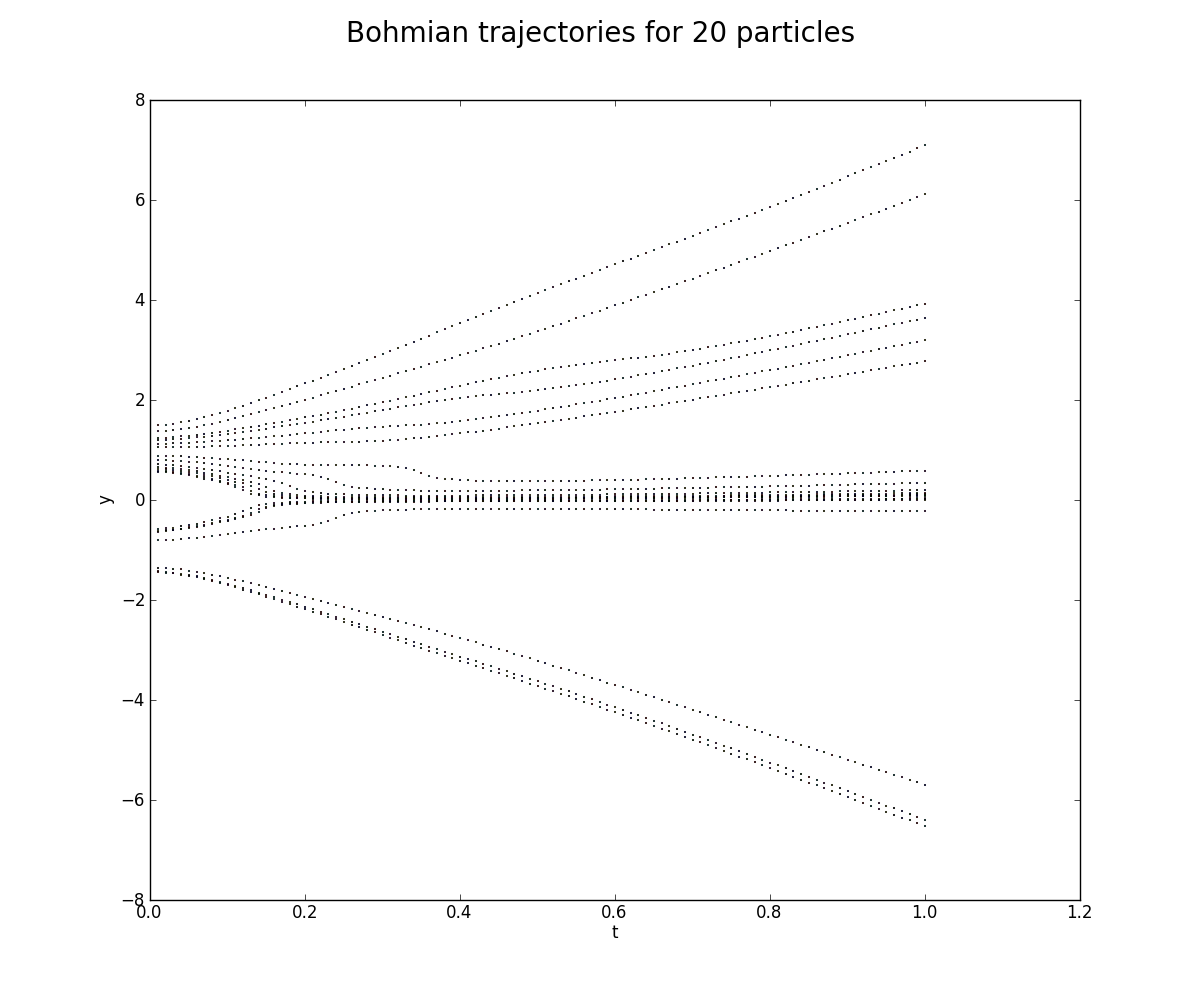
\includegraphics[scale=.3]{./imgs/20-particles-uniform-1.png}}
    \caption{
      20 particle trajectories with a random normal distribution.
      Note the interference pattern is already taking form.
    }
    \label{fig:trajsym}
  \end{figure}

  %Figure \ref{fig:trajsym} illustrates 50 trajectories calculated from a symmetrical, Gaussian distribution over each slit.
  %The symmetry is forced by calculating a random, Gaussian set over the first slit and mirroring these 25 points over the $y=0$ axis.
  %This gives the quintessential image of Bohmian trajectories for the double slit experiment (the original image can be found in reference \cite{philippidis}).
  %The trajectories follow distinct paths that differ from their classical counterparts. 
  %The trajectories are symmetrical about the axis between the slits and never cross each other's paths. 
  %There is also a definite interference pattern emerging when the time $t$ is one second. 

  %  [TODO: REMOVE SYM. FIGURE]
  \begin{figure}[!ht]
    \centerline{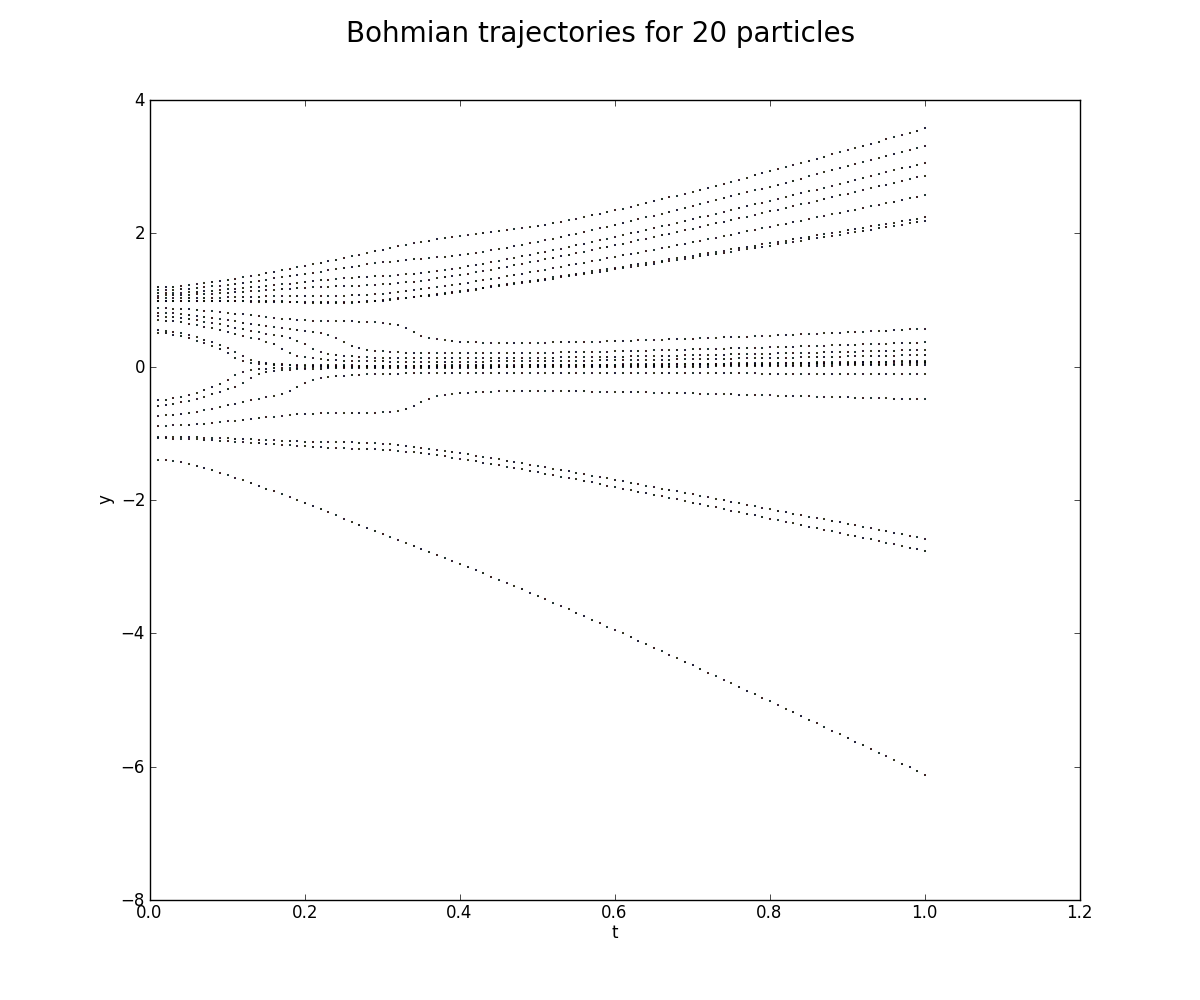
\includegraphics[scale=.3]{./imgs/20-particles-uniform-3.png}}
    \caption{
      20 particle trajectories with an random uniform distribution.
      Again, the interference pattern is already taking form.
    }
    \label{fig:trajnonsym}
  \end{figure}

  \begin{figure}[!ht]
    \centerline{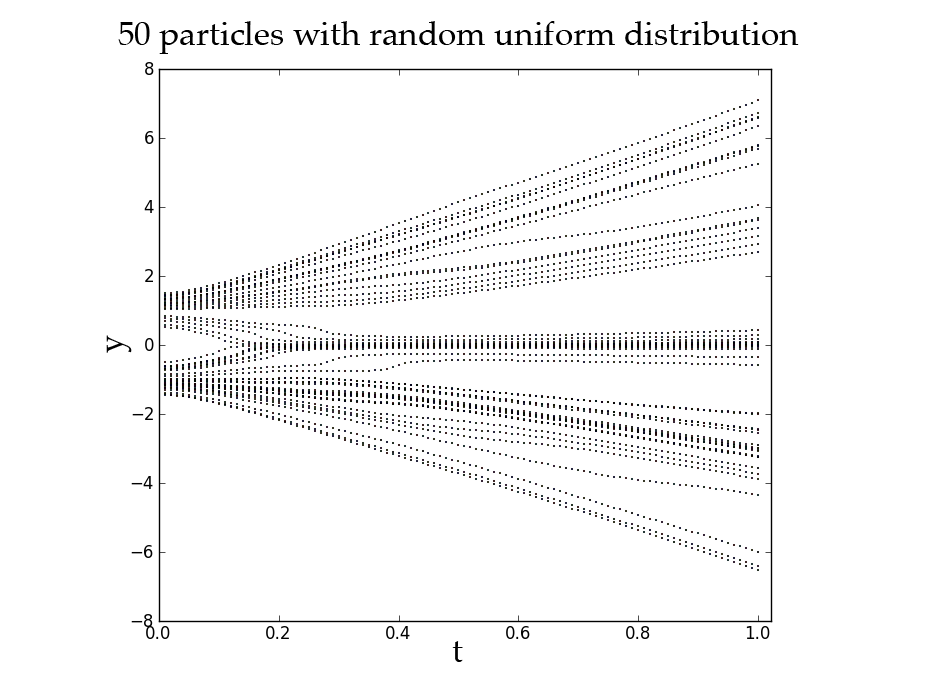
\includegraphics[scale=.5]{./imgs/50-particles-uniform.png}}
    \caption{
      50 particle trajectories with a random, uniform, non-symmetrical distribution over each slit.
      An interference pattern still occurs.
    }
    \label{fig:trajnorm}
  \end{figure}
  \nocite{philippidis}

  The basic criteria for Bohmian trajectories appear correct.
  There is a visual departure from classical trajectories in Figures \ref{fig:trajsym}, \ref{fig:trajnonsym} and \ref{fig:trajnorm} as well.
  Classically, if a particle starts at the slit with a distinct position and velocity it will continue along the direction of the
    particle's velocity in a straight line unless acted upon by an external force.
  %The depicted Bohmian interpretation do follow this classical description however not in classical form.
  The trajectories depicted do not follow straight paths and appear to veer at specific points.
  %These detours appear to be what causes the once straight paths to merge together and funnel themselves towards the screen
  %  in an what resembles an interference pattern.
  The cause of these detours is the quantum potential given by equation (\ref{eq:quantumpotential}).
  %The most convenient way of illustrating the effect is by evaluating the surface depicted in Figure \ref{fig:3d}.
  %If one imagines how a ball would travel along the surface, from the slits to the detector, the various rifts and valleys would detour
  %  the ball from a straight trajectory.
  %Note that Figure 3 does not depict the quantum potential which is the actual cause of the detours; however does provide a method for understanding the
  %  basic notion of why the particles follow the paths they do.
  %The particles are in fact acted upon by both the regular potential and quantum potential.
  %If the quantum potential existed classically as $\hbar \rightarrow 0$, the paths plotted in these figures would represent how objects would traverse classically.
  It provides a force, in the quantum realm, on the particles that govern the particles into trajectories foreign to classical behavior.
  %The quantum potential, however, is zero at the classical limit and therefore the trajectories plotted are foreign to classical behavior.
  %The only differing factor is the initial distribution of the particles: regarding either the number or position of the particles.
  Figures \ref{fig:trajsym} and \ref{fig:trajnonsym} also show an interference pattern taking shape even with just 20 particles in the system,
    which becomes a clearer interference pattern as more particles are introduced into the system.

  \begin{figure}
    \centerline{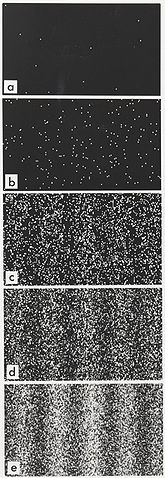
\includegraphics[scale=4.5]{./imgs/double-slit-results.jpg}}
    \caption{
    Screen results of the double slit experiment over time \cite{wiki}.
    }
    \label{fig:double-slit-results}
  \end{figure}

  %[TODO: TALK ABOUT THE SCREEN RESULTS OF THE DOUBLE SLIT EXPERIMENT]
  When this experiment is performed, Figure \ref{fig:double-slit-results} illustrates what a screen registers at different times.
  Both the Copenhagen and de Broglie-Bohm interpretations predict this interference pattern.
  The Copenhagen interpretation, however, ignores an explanation of the particle itself until it is measured by the screen, 
    while the de Broglie-Bohm interpretation offers a narrative of the particle's trajectory.
  As stated previously, a fundamental distinction is the de Broglie-Bohm notion that a single particle goes through a specific slit.
  The probability wave used in the Copenhagen interpretation does not quite offer this distinction and
    suggests that the particle goes through both slits and interferes with itself.
  The trajectories in Figures \ref{fig:trajsym} and \ref{fig:trajnonsym} would be representative of a screen at time $b$ in Figure \ref{fig:double-slit-results}, 
    while Figure \ref{fig:trajnorm} would be representative of a screen at time $c$.

\section{Secondary setup and trajectories}

  The Python class used to generate the previous trajectories is extended to fit a new wave function.
  Similar to the double-slit experiment, this secondary setup consists of a source that emits particles and a screen that captures the particle.
  Instead of the particle going through two slits, however, it hits a beam-splitter with 50\% chance of the particle going
    in one direction or another.
  After passing through the beam-splitter the particle hits a mirror and reflects towards the screen as illustrated in Figure \ref{fig:interfering-setup}.

  \begin{figure}[!ht]
    \centerline{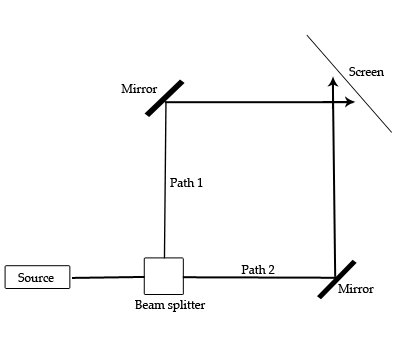
\includegraphics[scale=.6]{./imgs/secondary-setup.png}}
    \caption{
      The configuration setup for the interfering wave packet experiment.
    }
    \label{fig:interfering-setup}
  \end{figure}

  The wave packets are assumed to be Gaussian in nature and do not spread with time \cite{chaloupka}.
  Equation (\ref{eq:trajectories}) is used again to calculate the Bohmian trajectories for the wave function $\Psi$ that describes this system.
%  The only significant difference between this approach and that of the double-slit experiment is the wave function $\Psi$ and its behavior over time.
%  Besides $\Psi$, the general calculation of the Bohmian trajectories for interfering wave packets is the same.
  The contour plot shown in Figure \ref{fig:interfering} illustrates the wave function $\Psi$ at times $t=-15$, $t=0$ and $t=15$ seconds 
    as the wave packets $\psi_A$ and $\psi_B$ propagate towards each other on intersecting paths.
  %The contour plot demonstrates that these packets are three-dimensional in nature with their peak and highest curvature at the center.
  Initially, at $t=-15s$, the two wave packets are separate entities described by a single wave function traversing orthogonal paths.
  At $t=0$, the wave packets are completely superimposed upon each other forming an interference pattern with nodes and anti-nodes as the two Gaussian wave packets interfere.
  As the wave packets continue to propagate the interference pattern diminishes until eventually the wave packets are separate entities again;
    propagating along the same path as they initially were.
  The code to generate Figure \ref{fig:interfering} is shown in appendix \ref{appendix:contour-plot}.
  Code to generate a continuous animation of this contour plot is shown in appendix \ref{appendix:contour-plot-animated}.

%    [TODO: EXPLAIN EXPLAIN EXPLAIN THIS PLOT AND RELATE IT TO THE FIGURE SETUP]
  \begin{figure}[!ht]
    \centerline{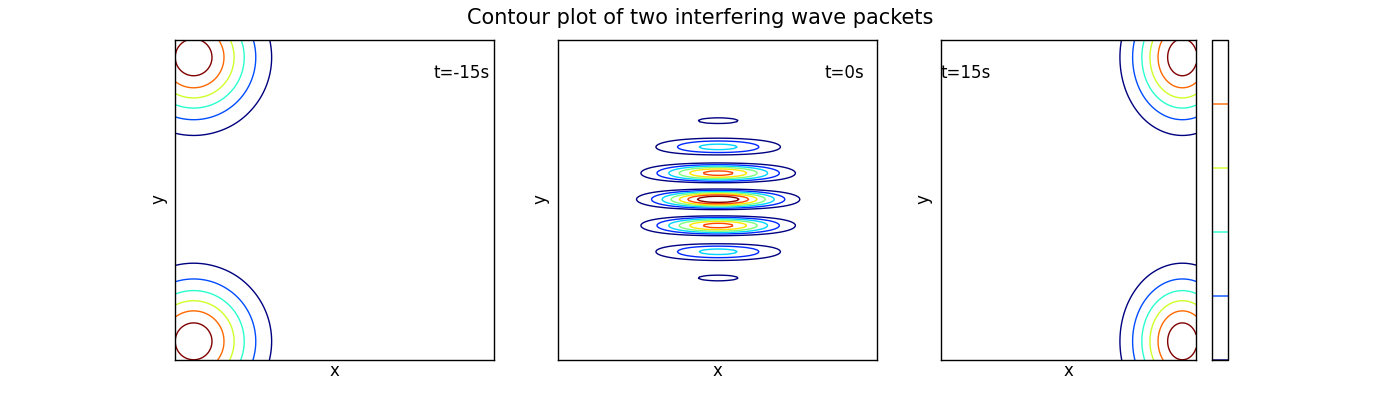
\includegraphics[width=\paperwidth]{./imgs/contour-plot.png}}
    \caption{
      Contour drawing of two interfering wave packets at times $t=-15s$, $t=0s$ and $t=15s$.
    }
    \label{fig:interfering}
  \end{figure}

%  The wave function that describes this system is given by the following equation \cite{chaloupka}
%  \begin{equation} 
%    \label{eq:interfering}
%    \begin{aligned}
%    \psi_A(\mathbf{r_x},\mathbf{r_y},t) = \exp \Bigg[  & i(k_0(\mathbf{r_x}\cos{\theta}-\mathbf{r_y}\sin{\theta})-ct)  \\
%                                                     &  -(\mathbf{r_x}\cos{\theta}-\mathbf{r_y}\sin{\theta})-ct)^2/a \\
%                                                     &  -(\mathbf{r_x}\sin{\theta}+\mathbf{r_y}\cos{\theta})^2/a  \Bigg]
%    \end{aligned}
%  \end{equation}
%  where $a$, $c$, $\theta$ and $k_0$ [TODO: WHERE THESE ARE WHAT?].
  %The variables $x$, $y$ and $t$ signify the positional coordinates and time evolution of the wave.
  %However, this only describes one of the wave packets $\psi_A$.
  %Given that both wave packets in Figure \ref{fig:interfering} show physical and behavioral symmetry over the center of the y-axis 
  %  the following symmetrical property can once again be assumed to find $\psi_B$
  %  [TODO: REMOVE SYM. EQUATION AGAIN]
  %\begin{equation}
  %  \psi_A(\mathbf{r_x},\mathbf{r_y},\mathbf{r_z},t) = \psi_B(\mathbf{r_x}, -\mathbf{r_y},\mathbf{r_z},t)
  %\end{equation}
  %just as in the double slit experiment.
  %Thereby giving equations for both wave packets $\psi_A$ and $\psi_B$ that yield an equation for the entire wave function of system via equation (\ref{eq:total-wave-function}).

  Calculating the Bohmian trajectories for the system yields the trajectories plotted in Figure \ref{fig:interfering-trajectories}.
  %The calculations were done under specific conditions. 
  The time $t$ spans from -15 seconds to 15 seconds with iterations of $0.1s$.
  The initial distribution of the particles is a random sampling of $y$ coordinates between -30 and 30 and initiate at time $t=-15s$.
  Plotting 20 trajectories takes approximately 6.2 seconds to compute.
  Once again the calculations find the $y$ coordinate of each particle since the $x$ coordinate is proportional to the time $t$.
  The Python code to generate Figure \ref{fig:interfering-trajectories} is shown in appendix \ref{appendix:secondary-trajectories} and is just an 
    extension of the Python class in appendix \ref{appendix:bohmian-trajectories} to accommodate the new wave function $\Psi$.
  %Other constants for the Gaussian function include: $a=36$, $c=1$, $\theta=\pi/4$ and $k_0=\pi\sqrt{2}/2$.
  %These values are chosen to emphasize the characteristics of the wave packets.
  %For example, a smaller value for $a$ shrinks the Gaussian wave packet and consequentially diminishes the effect on the Bohmian trajectories at the given resolution of Figure \ref{fig:interfering}. 
  %Other desired behaviors contributed to the value of the constants such as having [TODO: KEEP THIS?] $\psi_A$ and $\psi_B$ interfere at time $t=0s$ instead of time $t=15s$.
  %Granted these are subjected decisions but nonetheless have no effect on the general calculations of the Bohmian trajectories for this system.

  %A set of random particles are initially distributed along the $t=-15s$ axis.
  %In order to see the behavior of the Bohmian trajectories throughout the entire system the particles are distributed randomly, yet symmetrically, at values of $y$ between -30 and 30.
  %Although, the distribution can be limited to any portion of the $y$ axis if desired.
  %In regards to the computation time, a random set of fifty particles takes no longer then 15 seconds to calculate with the mentioned values above.

  %[TODO: REMOVE SYM.]
  \begin{figure}[ht]
    {\centering 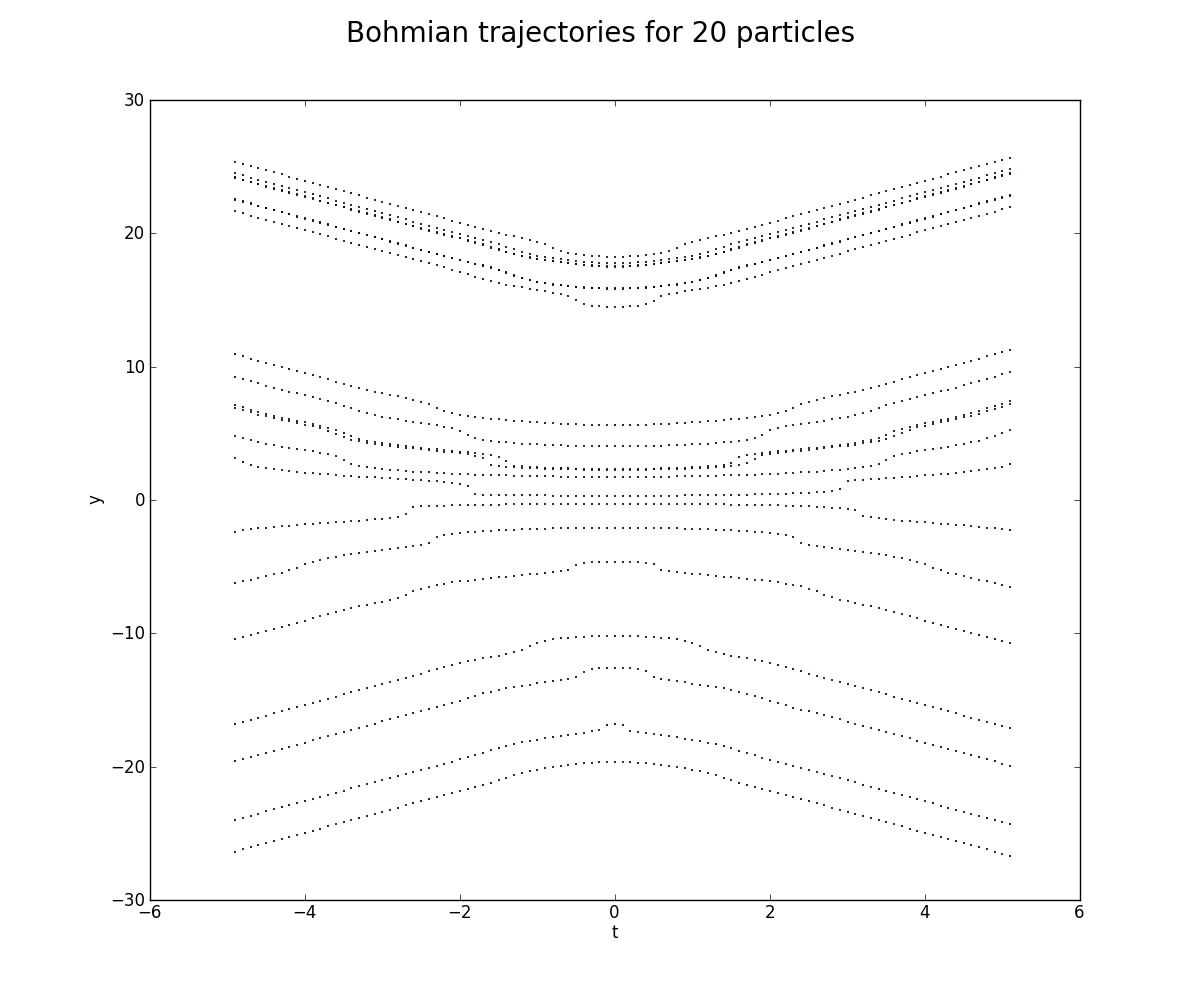
\includegraphics[scale=.4]{./imgs/interfering-trajectories.png} \\}
    \caption{
      Bohmian trajectories plotted for wave function $\Psi$ describing two interfering Gaussian wave packets.
      20 particles are initially distributed alone the $t=-15s$ axis ranging in values between -30 and 30.
      The trajectories do not cross paths nor the $y=0$ axis.
    }
    \label{fig:interfering-trajectories}
  \end{figure}

  %The results are [TODO: INTRIGUING IS WRONG WORD] intriguing and plotted in Figure \ref{fig:interfering-trajectories}. 
  An instinctive interpretation of the interfering wave packets depicted in Figure \ref{fig:interfering} can lead one to assume that the two wave packets 
    head towards each other, interfere with each other, and then continue along their original path.
  The Bohmian trajectories show that as the wave packets $\psi_A$ and $\psi_B$ begin to interfere with one another the Bohmian trajectories begin detouring.
  When the wave packets are fully superimposed at $t=0s$, the trajectories are almost parallel with the $t$ axis, never crossing the central line of symmetry at the $y=0$ axis. 
  As $\psi_A$ and $\psi_B$ continue propagating forward, the trajectories eventually turn around and head back towards the upper or lower region they originated from;
    creating another symmetry along the $t=0$ axis.
  This may indicate that the wave packets behave the same and just appear to continue along their original path.
  %The axis at $y=0$ behaves similar to an asymptotic limit for the trajectories. 
  The familiar characteristics of Bohmian trajectories are still observed: the trajectories do not cross and veer from classical trajectories.
  Also, regardless of the initial distribution of particles the trajectories follow the patterns illustrated in Figure \ref{fig:interfering-trajectories}.
  %That is to say that the $y=0$ and $t=0$ axis are axis of symmetry for the trajectories, which in fact never cross the $y=0$ axis.

  %In fact, if an initial particle is placed at $y=0$ it will propagate straight through the system as if the wave function does not exist.
  %This is illustrated in Figure \ref{fig:interfering-center}.

  %\begin{figure}
  %  {\centering \includegraphics[scale=.3]{./imgs/interfering-center.png} \\}
  %  \caption{
  %    A single particle placed initially at $y=0$ yields a straight path through the system not at all being affected by if the wave function $\Psi$.
  %  }
  %  \label{fig:interfering-center}
  %\end{figure}
%
%  Once again, the familiar characteristics of Bohmian trajectories are observed.
%  The Bohmian trajectories show a stark contrast to the assumed behavior of the wave packets.
%  Meaning, the trajectories do not continue on their initial direction after $t=0$ but in fact reverse it.
%  Regardless of the initial distribution of particles, the trajectories follow the same basic pattern as plotted in Figure \ref{fig:interfering-trajectories}.
%  Whichever side of the axis-of-symmetry the particle starts is where it remains throughout the system. 
%  The $y=0$ and $t=0$ axis are axis of symmetry for the trajectories, which in fact never cross the $y=0$ axis.
%  Furthermore, particles that initially start at $y=0$ will remain along this axis unimpeded.

\section{Conclusion}

  %[TODO: REMEMBER THESE ARE NOT SEPARATE SYSTEM. SAME SYSTEM, RELATED SYSTEMS BUT DIFFERENT SETUPS]
  In conclusion, Bohmian trajectories were numerically calculated with Python 2.7.2.
  A fourth-order Runge-Kutta was implemented to numerically solve the differential equation (\ref{eq:trajectories}) that describes the trajectories.
  Basic corroboration with known results was found regarding to the double-slit experiment.
  The expected interference pattern was observed and the effects of the quantum potential were noticeable through the deviations in the trajectories from their classical counterparts.
  All the Python scripts are referenced in the appendix and have the NumPy, SymPy and Matplotlib packages as dependencies.
  Computation times were relatively quick and given the open-sourced foundation of Python and its scientific packages the results can be freely replicated.
  %The first system being the double-slit experiment and the second being two interfering wave packets.
  %Each system displays different trajectories but the core characteristics of the trajectories are similar.
  %Python was the language of choice and proved sufficient in delivering the calculations and graphs necessary to investigate the two systems.
  %Different initial distributions of particles were implemented and they all demonstrated unique trajectories that obeyed the characteristics of Bohmian trajectories and 
  %  the reality of the double-slit experiment.

  %In regards to the interfering wave packets, Bohmian trajectories were again discovered to obey their intrinsic characteristics.
  %However, this had some unique consequences in the paths of the trajectories.
  %Specifically, particles that initially start with positive $y$ coordinates would follow a trajectory that never cross the $y=0$ axis.
  %Coordinates initially with negative $y$ values would follow [TODO: WHAT DOES THIS MEAN? KEEP IT?] the same behavior.
  %Particles that initially started at $y=0$ would remain on the $y=0$ axis and never deviate from it.
  %Again, the computation times were rather quick making higher precision modeling for this system possible as well.

  %Although minor changes may have to be made to the code in this case.

%  Bohmian mechanics offers a different perspective on modern quantum mechanic theory.
%  By prescribing definite trajectories to the particles, the notion of wave-particle duality is omitted at the expense of the quantum potential being introduced.
%  It is well known that the Bohmian perspective has not yet offered alternate answers or predictions, however,
%    it does provide an alternative explanation of quantum mechanic behavior that is not completely foreign to the classical world.
%  [TODO: REMOVE THE SUPERFULOUS LINE] It would then seem justified to continue investigating this alternative perspective of quantum mechanics.
%  
%  [todo: compare to current dBB stuff, that's what the conclusion should be about. talk about the python more. why it's good to use. debugging, syntax, accessible to anyone etc..]
  

  

\pagebreak

\bibliographystyle{plain}
\bibliography{sources}

\pagebreak

\appendix
\newgeometry{left=2cm,right=2cm}

\section{Real and imaginary parts of the wave function for the double slit system}
\label{appendix:real-imag}
\verbatiminput{scripts/real-imaginary-graphs.py}
\pagebreak

\section{Imaginary surface over time of the wave function for a double slit system}
\label{appendix:imaginary-surface}
\verbatiminput{scripts/imaginary-surface.py}
\pagebreak 

\section{Bohmian trajectories for the double-slit setup}
\label{appendix:bohmian-trajectories}
\verbatiminput{scripts/bohm.py}
\pagebreak 

\section{Contour plot}
\label{appendix:contour-plot}
\verbatiminput{scripts/second-contour.py}
\pagebreak 

\section{Animated contour plot}
\label{appendix:contour-plot-animated}
\verbatiminput{scripts/second-contour-animated.py}
\pagebreak 

\section{Bohmian trajectories for the second setup}
\label{appendix:secondary-trajectories}
\verbatiminput{scripts/second.py}
\pagebreak 


\end{document}
